\documentclass[14pt,a4paper,article,oneside]{ncc}
\usepackage[a4paper,left=3cm,right=1.5cm,top=2cm,bottom=2cm]{geometry}
\usepackage{amsmath}
\usepackage{amsfonts}
\usepackage[T2A]{fontenc}
\usepackage[utf8]{inputenc}
\usepackage[english,russian]{babel}
\usepackage{indentfirst}
\usepackage{graphicx}
\usepackage{float}

\usepackage{fancyhdr}
\pagestyle{plain}


\usepackage{listings}

\begin{document}
% Title page
    \begin{titlepage}
        \thispagestyle{empty}
        \begin{center}
            \textsc{
                Санкт-Петербургский политехнический университет имени Петра Великого \\[5mm]
                Институт прикладной математики и механики\\[2mm]
                Высшая школа прикладной математики и физики
            }
            \vfill
            \textbf{\large
            Направление подготовки\\
            «01.03.02 Прикладная математика и информатика»\\[3mm]
            }
            \vfill
            \textbf{\large
            Курсовая работа «Сравнительный анализ градиентных методов второго порядка»\\[5mm]
            Дисциплина «Методы оптимизации»\\
            }
        \end{center}

        \vfill

        \begin{minipage}{0.5\textwidth}
            \begin{flushleft}
                Выполнили студенты группы\\5030102/90201:
            \end{flushleft}
        \end{minipage}
        \begin{minipage}{0.5\textwidth}
            \begin{flushright}
                Габдушев Р.М.\\
                Фисюк А.Ю.\\
                Ахметшин Р.И.
            \end{flushright}
        \end{minipage}\\\\\\
        \begin{minipage}{0.5\textwidth}
            \begin{flushleft}
                Преподаватель:
            \end{flushleft}
        \end{minipage}
        \begin{minipage}{0.5\textwidth}
            \begin{flushright}
                Родионова Е.А.
            \end{flushright}
        \end{minipage}\\

        \vfill

        \begin{center}
            Санкт-Петербург\\
            \theyear\ г.
        \end{center}

    \end{titlepage}

    \tableofcontents
    \newpage
    \listoffigures

    % Введение
    \newpage
    \section{Введение}
\label{sec:introduction}
Проблема оптимизации функций многих переменных имеет приложения во всех сферах, где используются математическое моделирование в любом виде.

Задачи линейного программирования - простейший класс таких задач, широко распространён на практике, хорошо изучен и имеет эффективные методы решения.

Однако, список задач, требующих оптимизации, выходит далеко за эти рамки.
И не каждая этих них может похвастаться настолько эффективными методами решения.

В этой работе мы рассмотрим класс задач выпуклой оптимизации, а именно оптимизация функций нескольких переменных, без ограничений.

Целью работы является сравнительный анализ градиентных методов второго порядка:

\begin{itemize}
    \item Градиентный метод Ньютона
    \item Градиентный метод Ньютона с дроблением шага (Пшеничного)
    \item Градиентный метод Бройдена - Флетчера - Гольдфарба - Шанно(БФГШ)
\end{itemize}


В частности:
\begin{itemize}
    \item найти ориентировочную вычислительную сложность на один наг алгоритма
    \item привести графическую иллюстрацию хода работы методов
    \item провести сравнение скорости сходимости на наборе показательных функций
    \item вынести рекомендации о выборе метода, в зависимости от особенностей функции
\end{itemize}



    % Постановка задачи
    \newpage
    \section{Постановка задачи}
\label{sec:problem}
\noindent Дана функция
\begin{equation}
    f:\mathbb{R}^{n} \rightarrow \mathbb{R}
\end{equation}

\noindent Найти
\begin{equation}
    x_n \in B(\epsilon, x_*):  f(x_*) = \min_{x \in \mathbb{R}^{n}} f(x)
\end{equation}
\noindent где $\epsilon > 0$ - заданная точность.

    % Описание методов
    \section{Описание методов}
\label{sec:methods}

Градиентные методы основаны на идее аппроксимации минимизируемой функции её разложением в текущей точке, удерживая члены до определённого порядка.
В случае методов второго порядка, аппроксимация функции $f$ в точке $x_k$ выглядит так:
\begin{equation}
    f(x) \approx f(x_k) + \nabla^{T}f(x_k)(x - x_k) + (x - x_k)^{T}H(x_k)(x - x_k)/2
    \label{eq:taylor_decomposition}
\end{equation}
\noindent где $\nabla{f(x_k)}$ - значение градиента, а $H(x_k)$ - матрица Гессе, в точке разложения.\\
Предполагая, что данная функция принадлежит по крайней мере $C^2$ и выпукла, делаем вывод, что и её приближение выпукло.
Значит оно имеет единственный минимум $x_*$.[3]\\
Из \eqref{eq:taylor_decomposition} элементарно вычисляется оптимизирующий вектор $p_k = x_* - x_k$:\\
\begin{equation}
    p_k = -(H(x_k))^{-1}{\nabla}f(x_k)
    \label{eq:aprox_optim_vector}
\end{equation}

\subsection{Градиентный метод Ньютона}
\label{subsec:theory_newton}

Метод ньютона предполагает следующее правило построения минимизирующей последовательности:
\begin{enumerate}
    \item $x_k = x_0$
    \item Если условие окончания не выполнено - дальше
    \item $p_k = -(H(x_k))^{-1}{\nabla}f(x_k)$
    \item $x_{k+1} = x_k + p_k$
    \item  $k = k + 1$
    \item Возврат к пункту 2
\end{enumerate}
$x_0$ - начальное приближение

\subsection{Градиентный метод Ньютона с дроблением шага (Пшеничного)}
\label{subsec:theory_pschen}
Данная модификация метода Ньютона предлагает перед переходом к следующему шагу,
дробить длину шага пока не будет выполнено особое условие.

Алгоритм построения последовательности:
\begin{enumerate}
    \item $x_k = x_0$
    \item Если условие окончания не выполнено - дальше
    \item $p_k = -(H(x_k))^{-1}{\nabla}f(x_k)$
    \item $\alpha = 1$
    \item Если $f(x_k + \alpha p_k) - f(x_k) \leq \alpha \delta \nabla^{T}f(x_k)p_x$ - переход к пункту 6
    \item $\alpha = \alpha \lambda$
    \item Возврат к пункту 5
    \item $x_{k+1} = x_k + \alpha p_k$
    \item Возврат к пункту 2
\end{enumerate}
$x_0$ - начальное приближение, $0 <\delta\leq \frac{1}{2}, 0 <\lambda <1$ - параметры дробления.

\subsection{Градиентный метод БФГШ}
\label{subsec:theory_bfgs}
В приложениях исходная функция, как правило, не задаётся формулой, а определяется в ходе измерений.
Поэтому матрицу Гессе тоже не получить символьно, а её вычисление требует довольно много обращений к функции.
К тому же на каждом шаге необходимо её обращать.

Градиентный метод Бройдена - Флетчера - Гольдфарба - Шанно(БФГШ) относится к квазиньютоновским и помогает обойти эти трудности.

Вместо точного вчисления матрицы Гессе и её обращения, строится последовательность матриц, которая  [1] сходится к обращённой матрице гессе.

Схема вычисления[1]:
\begin{equation}
C_{k + 1} = (I - \rho_k s_k y_k^T)C_k(I - \rho_k y_k s_k^T) + \rho_k s_k s_k^T,
\label{eq:bfgs_mat}
\end{equation}
где $\rho_k = \frac{1}{y_k^T s_k}$, $I$ - единичная матрица, $s_k = x_{k + 1} - x_k$ - шаг алгоритма на итерации, $y_k = \nabla f_{k + 1} - \nabla f_{k}$ - изменение градиента на итерации.
В качестве начального приближения матрицы можно взять единичную.

Также такая матрица обладает свойством самокоррекции, если длина шага выбирается одномерным поиском минимума функции по найденному направлению $p_k$:

\begin{equation}
f(x_k + \alpha_k p_k) = min_{\alpha \geq 0} f(x_k + \alpha p_k)
\end{equation}

В итоге алгоритм выглядит следующим образом:

\begin{enumerate}
    \item $x_k = x_0$
    \item $C_k = C_0$
    \item Если условие окончания не выполнено - дальше
    \item $p_k = -(C_k){\nabla}f(x_k)$
    \item $\alpha = 1$
    \item Поиск оптимального $\alpha_x f(x_k + \alpha_k p_k) = min_{\alpha \geq 0} f(x_k + \alpha p_k)$
    \item $s_k = \alpha p_k$
    \item $x_{k+1} = x_k + s_k$
    \item Обновить $C_{k+1}$ по формуле \eqref{eq:bfgs_mat}
    \item Возврат к пункту 2
\end{enumerate}

Для всех методов существуют вариации, в которых матрица вычисляется не на каждом шаге, но в нашей работе мы вычисляем её каждый раз.

    % Выбор функций для оптимизации
    \newpage
    \section{Выбор функций для оптимизации}
\label{sec:functions}

Для наглядной графической иллюстрации работы методов, мы будем оптимизировать функции двух переменных.

\begin{enumerate}

    \item Рассмотрим функцию второго порядка:
    \begin{equation}
        f_1(x, y) = 2x^2 + y^2 + xy
        \label{eq:func_1}
    \end{equation}

    Минимум этой функции методы второго порядка в идеале должны находить за один шаг.

    \item Также рассмотрим функцию, состоящую из членов разложения степени выше второй
    \begin{equation}
        f_2(x, y) = x^4 + (\frac{y}{2})^4
        \label{eq:func_2}
    \end{equation}

    \item Ещё рассмотрим эту же функцию, но с добавлением квадратичных членов:
    \begin{equation}
        f_3(x, y) = x^4 + (\frac{y}{2})^4 + (\frac{x}{2})^2 + y^2
        \label{eq:func_3}
    \end{equation}

    \item Также, рассмотрим функцию, включающую степени выше 2 с малыми коэффициентами:
    \begin{equation}
        f_4(x, y)=x^{2}+y^{2}+0.05(x^{4}+y^{4})+0.0025(x^{6}+y^{6})+x+y
        \label{eq:func_4}
    \end{equation}

\end{enumerate}

    % Применимость методов
    \section{Применимость методов}
\label{sec:applicability}

Градиентные методы второго порядка применимы к строго выпуклым, дважды непрерывно дифференцируемым функциям.[2]
Покажем, что это верно для выбранных функций, приведя их градиенты и матрице Гессе:

\begin{equation}
    \nabla f_1(x, y) = (4x + y,  2y + x)
    \label{eq:func_1_grad}
\end{equation}

\begin{equation}
    H_1(x, y) =
    \begin{pmatrix}
        4 & 1\\
        1 & 2
    \end{pmatrix}
    \label{eq:func_1_hesse}
\end{equation}

\begin{equation}
    \nabla f_2(x, y) = (
        4x^3,  \frac{1}{4}y^3
    )
    \label{eq:func_2_grad}
\end{equation}

\begin{equation}
    H_2(x, y) =
    \begin{pmatrix}
            12 x^2 & 0\\
            0 & \frac{3}{4}y^2
    \end{pmatrix}
    \label{eq:func_2_hesse}
\end{equation}

\begin{equation}
    \nabla f_3(x, y) = (4x^3 + \frac{x}{2},  \frac{y^3}{4} + 2y)
    \label{eq:func_3_grad}
\end{equation}

\begin{equation}
    H_3(x, y) =
    \begin{pmatrix}
        12 x^2 + \frac{1}{2} & 0\\
        0 & 3\frac{y^2}{4} + 2
    \end{pmatrix}
    \label{eq:func_3_hesse}
\end{equation}

\begin{equation}
    \nabla f_4(x, y) = (0.0015x^5 + 0.02x^3 + 2x + 5,  0.0015y^5 + 0.02y^3 + 2y + 5)
    \label{eq:func_4_grad}
\end{equation}

\begin{equation}
    H_4(x, y) =
    \begin{pmatrix}
        0.0075x^4 + 0.6x^2 + 2 & 0\\
        0 & 0.0075y^4 + 0.6y^2 + 2
    \end{pmatrix}
    \label{eq:func_4_hesse}
\end{equation}

Видим, что все функции выпуклые, и все, кроме $f_2$ - строго выпуклые.
Рассмотрим поведение методов на нестрого выпуклых функциях, а потому не будем исключать $f_2$.

    % Результаты
    \newpage
    \section{Результаты}
\label{sec:results}

Для начала проведём вычисления с использованием малости нормы градиента в качестве критерия остановки.

Вычисления проводились для точности $10^{-6}$, параметры дробления метода Пшеничного: $\lambda = 0.9, \epsilon = 0.45$

Далее приведены графики зависимости точности (нормы разности текущего и точного значения) от номера шага и геометрическая интерпретация работы методов (показаны линии уровня и вектора шага).

Здесь и далее, графики в логарифмическом размере выглядят вертикальными, если принимают значение 0 (точное решение).

Зелёный пунктир - заданная точность

\begin{figure}[H]
			\centering
			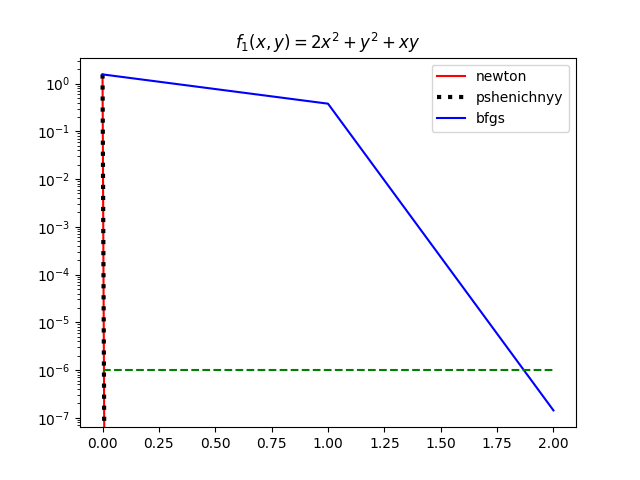
\includegraphics[scale=0.75]{figures/acc_from_step_func1}
			\caption{Точность от шага, $f_1$, критерий - градиент}
			\label{fig:acc_from_step_func1}
\end{figure}

\begin{figure}[H]
			\centering
			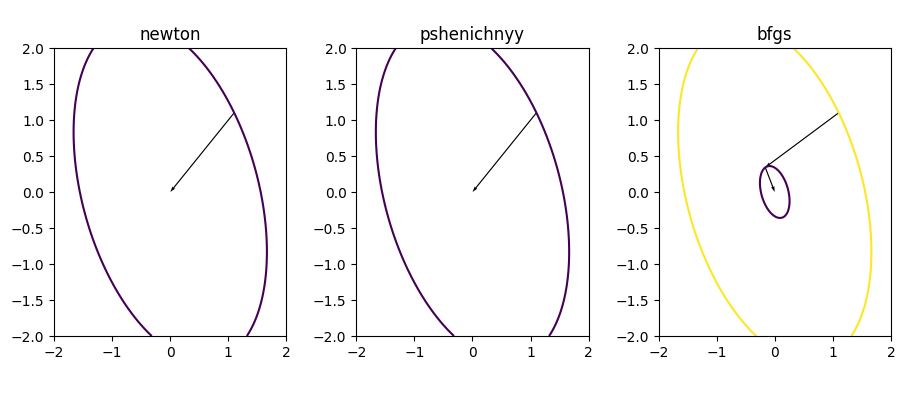
\includegraphics[scale=0.75]{figures/process_view_func1}
			\caption{Иллюстрация работы алгоритмов, $f_1$}
			\label{fig:process_view_func1}
\end{figure}

Как видим, заданная точность достигается всеми алгоритмами, остановка происходит вовремя.
Как и ожидалось, методы второго порядка решили точно за 1 шаг.
Квазиньютоновский метод очень хорошо приблизил решение на втором шаге (сразу после первой корректировки приближения матрицы Гессе)

\begin{figure}[H]
			\centering
			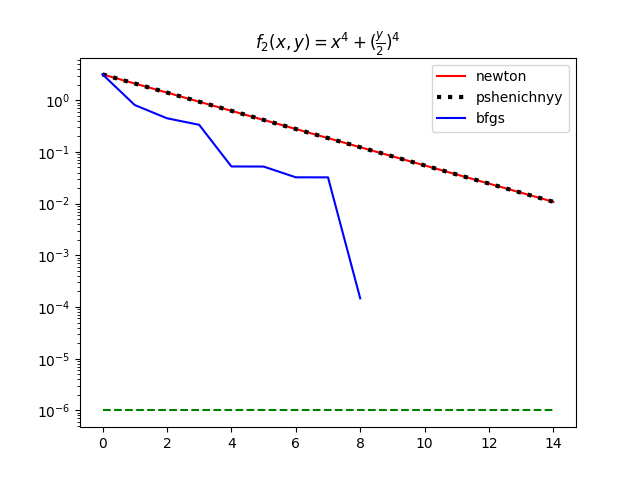
\includegraphics[scale=0.75]{figures/acc_from_step_func2}
			\caption{Точность от шага, $f_2$, критерий - градиент}
			\label{fig:acc_from_step_func2}
\end{figure}

\begin{figure}[H]
			\centering
			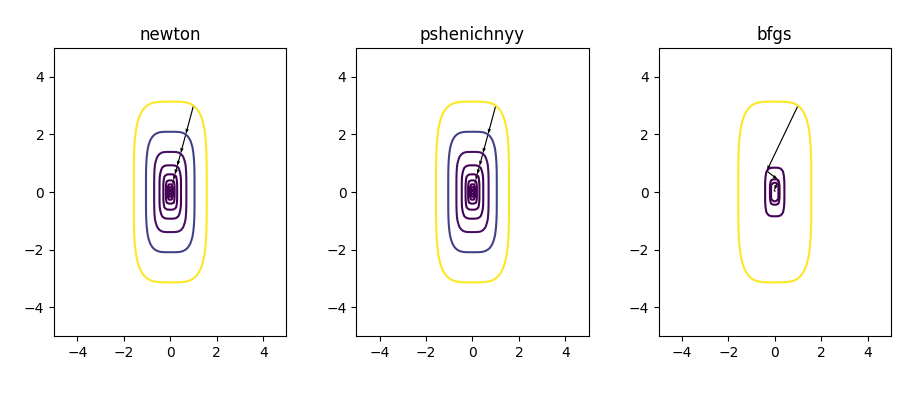
\includegraphics[scale=0.75]{figures/process_view_func2}
			\caption{Иллюстрация работы алгоритмов, $f_2$}
			\label{fig:process_view_func2}
\end{figure}

Заметим, что так как в окрестности точки минимума функция ведёт себя как функция четвёртой степени, градиентная оценка приводит к преждевременной остановке алгоритма.

Также, этот опыт показывает, что данная функция плохо аппроксимируется эллиптическим параболоидом, поэтому методы второго порядка медленно сходятся.
Квазиньютоновский метод в этом случае оказывается быстрее, благодаря оптимальному выбору длины шага.

\begin{figure}[H]
			\centering
			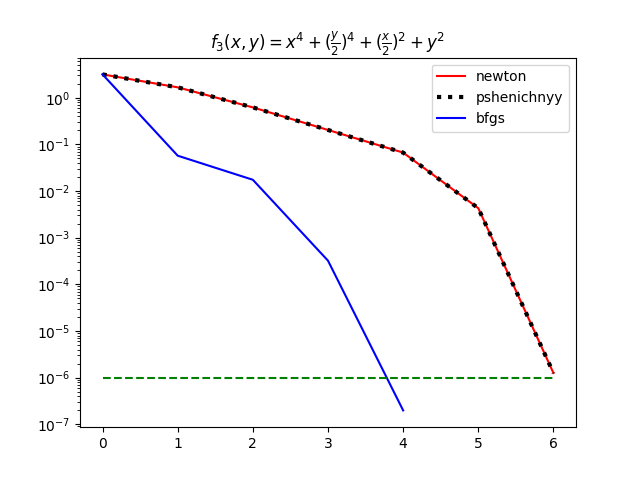
\includegraphics[scale=0.75]{figures/acc_from_step_func3}
			\caption{Точность от шага, $f_3$, критерий - градиент}
			\label{fig:acc_from_step_func3}
\end{figure}

\begin{figure}[H]
			\centering
			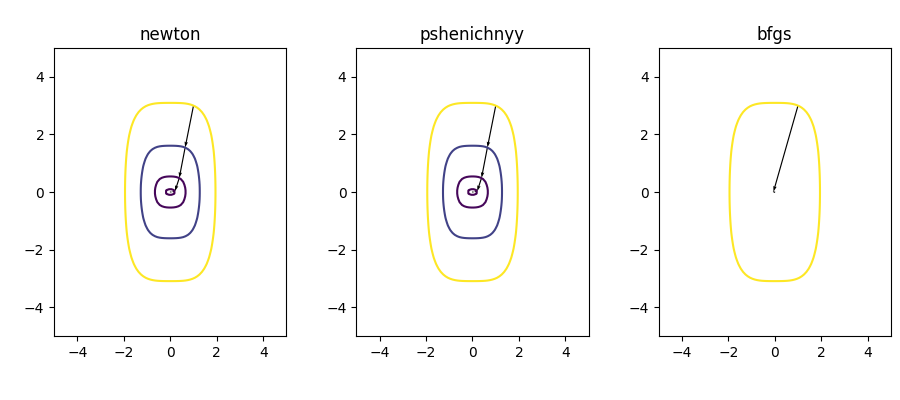
\includegraphics[scale=0.75]{figures/process_view_func3}
			\caption{Иллюстрация работы алгоритмов, $f_3$}
			\label{fig:process_view_func3}
\end{figure}

Видим, что при добавлении к $f_2$ квадратных членов достоверность градиентного критерия улучшилась, хотя и не полностью, так как методы второго порядка хоть и приблизились близко, но не дали заданной точности.

Одновременно с этим, все методы стали сходиться быстрее, но квазиньютоновский метод всё ещё обходит квадратичные.

\begin{figure}[H]
			\centering
			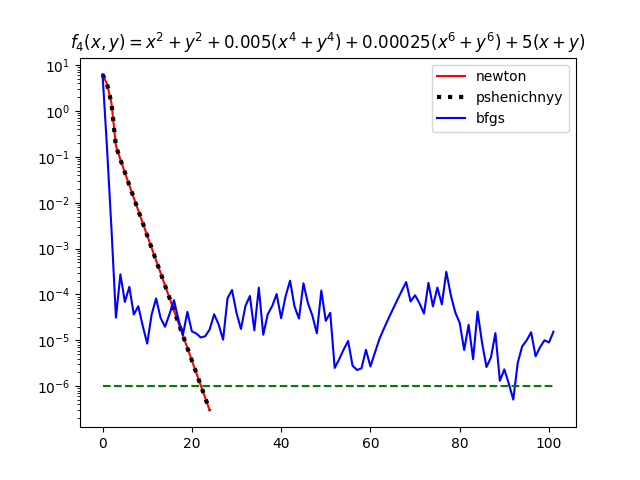
\includegraphics[scale=0.75]{figures/acc_from_step_func4}
			\caption{Точность от шага, $f_4$, критерий - градиент}
			\label{fig:acc_from_step_func4}
\end{figure}

\begin{figure}[H]
			\centering
			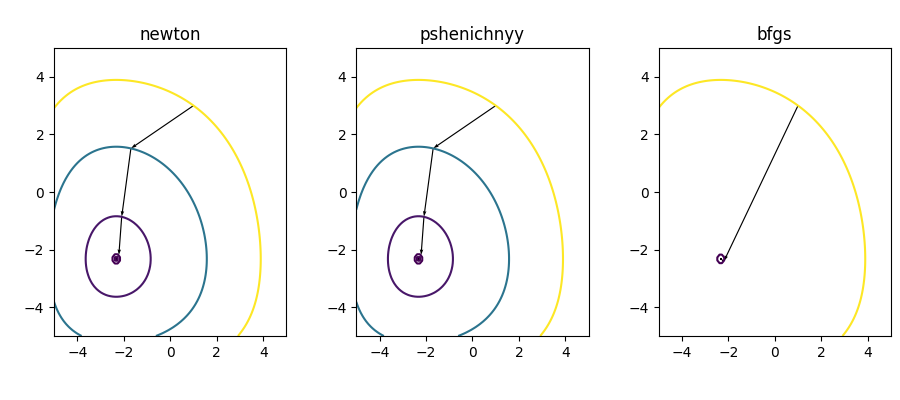
\includegraphics[scale=0.75]{figures/process_view_func4}
			\caption{Иллюстрация работы алгоритмов, $f_4$}
			\label{fig:process_view_func4}
\end{figure}

Как видим, на данной функции квадратичные методы сходятся медленнее, чем в случае $f_3$, а квазиньютоновский и вовсе перестаёт сходиться ближе $10^-4$.

Отметим, что эта функция единственная из рассмотренных с минимумом не в нуле.
Но, проведя исследования этой же функции с перенесённым в точку минимума началом координат, мы увидели абсолютно те же результаты.

Градиентная оценка здесь приводит к нескольким лишним шагам алгоритма.



Как показал этот опыт, на выбранных нами функциях метод Пшеничного всегда выполняет 0 дроблений и вырождается в метод Ньютона, поэтому далее не будем его рассматривать.

В следующем опыте проверим скорость сходимости методов, в зависимости от начального приближения.
Для этого проведём вычисления для 100 точек, равномерно распределённых на окружности с центром в точке минимума и радиусом 2.
На следующих графиках изображена зависимость близости решения от номера шага алгоритма.
В этом опыте критерием остановки взято расстояние до точного решения, так как ранее было показано, что градиентный критерий даёт разные результаты для разных функций.

На рисунках красным обозначены решения методом Ньютона, синим - методом БФГШ.
Зелёным пунктиром отмечена целевая точность $= 10^-6$.

\begin{figure}[H]
			\centering
			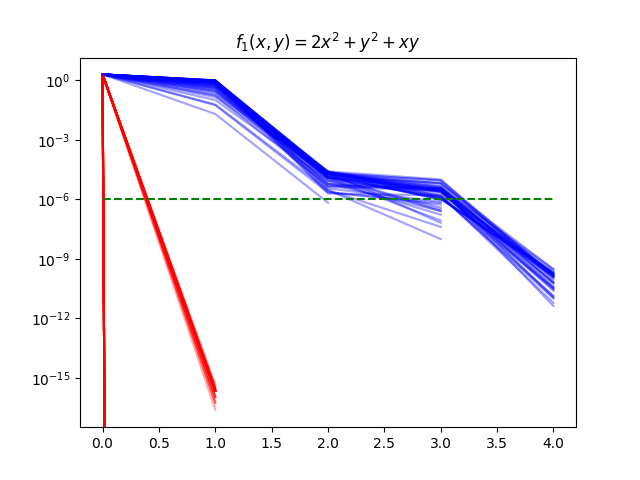
\includegraphics[scale=0.75]{figures/init_100_func1}
			\caption{Выборка начальных приближений, $f_1$}
			\label{fig:init_100_func1}
\end{figure}

Для первой функции метод Ньютона всегда находит решение за 1 шаг, в некоторых случаях - точно (вертикальные линии на графике).
Квазиньютоновскому методу требуется от 2 до 4 шагов.
В среднее число шагов в выборке 3,7.

\begin{figure}[H]
			\centering
			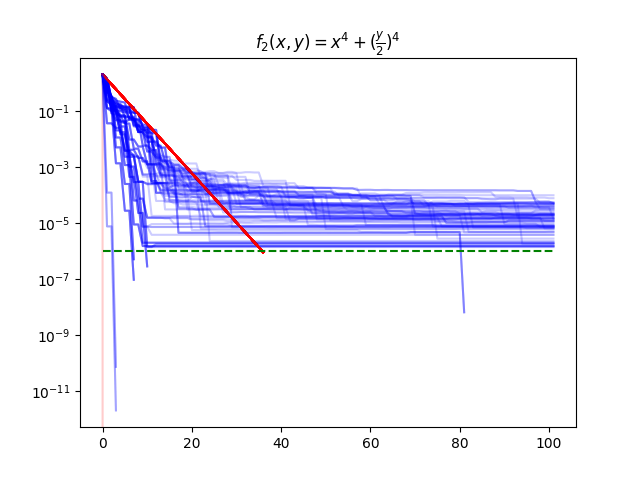
\includegraphics[scale=0.75]{figures/init_100_func2}
			\caption{Выборка начальных приближений, $f_2$}
			\label{fig:init_100_func2}
\end{figure}

Здесь становится видно, квазиньютоновский метод плохо справляется с полиномами 4 степени и не сходится в большинстве случаев.
Метод ньютона же, сходится за 36 шагов, и обладает зависимостью $n = -5,7 log_10(|x_*-x|)$.

\begin{figure}[H]
			\centering
			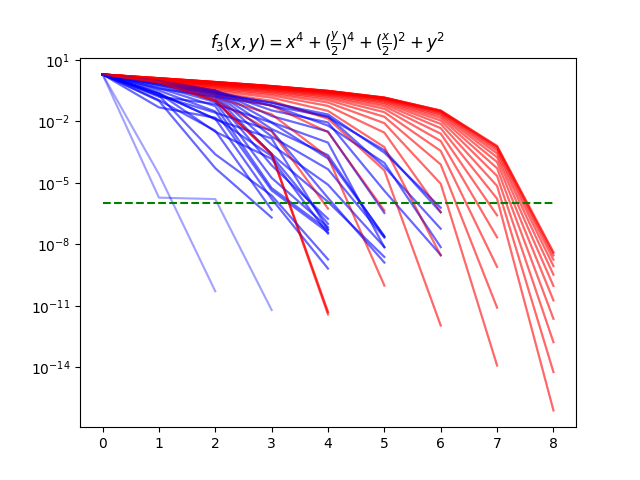
\includegraphics[scale=0.75]{figures/init_100_func3}
			\caption{Выборка начальных приближений, $f_3$}
			\label{fig:init_100_func3}
\end{figure}

При добавлении квадратичных членов оба метода стали хорошо сходиться.
Но при этом, для данной функции наблюдается заметный разброс в скорости сходимости от начального приближения для обоих методов.
Среднее число шагов:

Метод ньютона - 6.76

Метод БФГШ - 4.58

\begin{figure}[H]
			\centering
			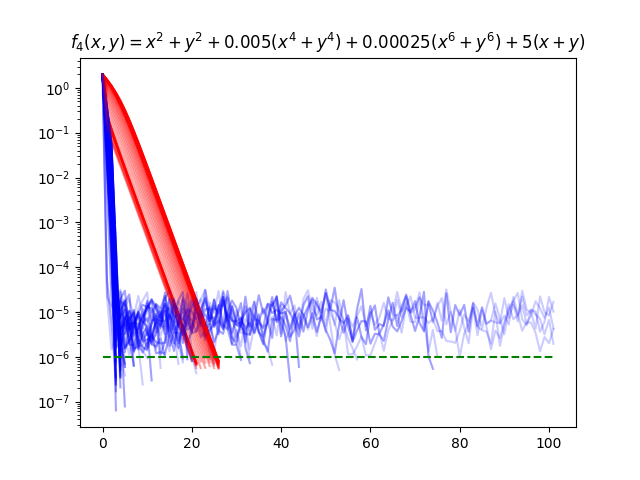
\includegraphics[scale=0.75]{figures/init_100_func4}
			\caption{Выборка начальных приближений, $f_4$}
			\label{fig:init_100_func4}
\end{figure}

Для данной функции снова имеем не сходящийся ближе чем $10^-5$ метод БФГШ и зависимость $n = a+b log_10(|x_*-x|)$.
Однако, в отличие от функции $f_2$, где БФГШ не ухудшал результат, здесь явно видны скачки точности в худшую сторону.


    % Заключение
    \newpage
    \section{Заключение}
\label{sec:conclusion}
В ходе работы было показано, что квазиньютоновские методы могут показывать себя лучше Ньютоновских на определённых задачах, а также позволяют не вычислять вторые производные, что очень полезно, если функция вычисляется трудозатратно. Однако, в ряде других случаев, метод БФГШ вообще не может достичь поставленной точность, тогда как Ньютоновский метод сходится. Таким образом, имеет смысл сначала использовать метод БФГШ, а после достаточного приближения к точке, переходить на метод Ньютона.

Что касается метода Пшеничного, нам не удалось найти строго выпуклые функции, на которых он вёл бы себя отлично от метода Ньютона, но это не значит, что их нет.


    % Список литературы
    \newpage
    \section{Список литературы}
\label{sec:literature}
\begin{enumerate}
    \item Bonnans, J. Frédéric; Gilbert, J. Charles; Lemaréchal, Claude; Sagastizábal, Claudia A., "Newtonian Methods", Numerical Optimization: Theoretical and Practical Aspects (Second ed.), Berlin: Springer, 2006. pp. 51–66
    \item Базара М., Шетти К. Нелинейное программирование.-М.: Мир, 1982.- 583 с.
    \item Болдырев Ю. Я., Родионова Е. А. Методы оптимизации. Математическое программирование: Учеб. пособие СПб.: Изд-во СПбГТУ, 1999. 82 с.
\end{enumerate}



\end{document}